\usetikzlibrary{patterns}
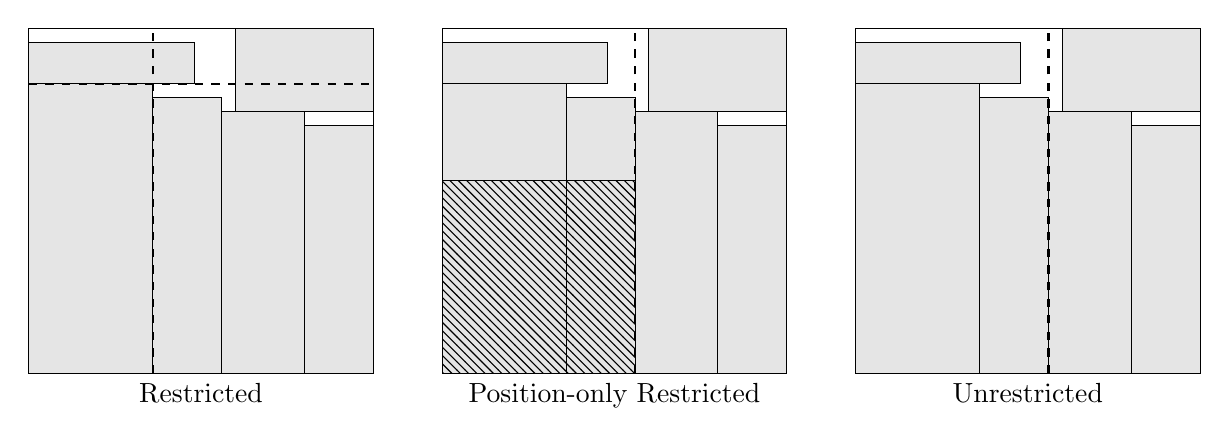
\begin{tikzpicture}[scale=0.175]
\def\piececolor{gray!20}
\def\labelxshift{12.5}
\def\labelyshift{0}
\def\labelfontsize{\normalsize}

\begin{scope}[shift={(0, 0)}] % FIRST ROW
\begin{scope}[shift={(0, 0)}] % FIRST IMAGE
\draw (0,0) rectangle +(25, 25);

%\draw[fill=\piececolor] (0,0) rectangle +(6, 19);
%\draw[fill=\piececolor] (6,0) rectangle +(5, 18);
\draw[fill=\piececolor] (14,0) rectangle +(6, 19);
\draw[fill=\piececolor] (20,0) rectangle +(5, 18);
\draw[fill=\piececolor] (0,0) rectangle +(9, 21);
\draw[fill=\piececolor] (9,0) rectangle +(5, 20);
%\draw[fill=\piececolor] (0,19) rectangle +(10, 6);
\draw[fill=\piececolor] (15,19) rectangle +(10, 6);
\draw[fill=\piececolor] (0,21) rectangle +(12, 3);

\draw[dashed, thick, black] (0, 21) -- (25, 21);
\draw[dashed, thick, black] (9, 0) -- (9, 25);


\node [below] at (\labelxshift, \labelyshift) {\labelfontsize Restricted};


\draw (0,0) rectangle +(25, 25);
\end{scope}

\begin{scope}[shift={(30, 0)}] % SECOND IMAGE
\draw (0,0) rectangle +(25, 25);

%\draw[fill=\piececolor] (0,0) rectangle +(6, 19);
%\draw[fill=\piececolor] (6,0) rectangle +(5, 18);
\draw[fill=\piececolor] (14,0) rectangle +(6, 19);
\draw[fill=\piececolor] (20,0) rectangle +(5, 18);
\draw[fill=\piececolor] (0,0) rectangle +(9, 21);
\draw[fill=\piececolor] (9,0) rectangle +(5, 20);
%\draw[fill=\piececolor] (0,19) rectangle +(10, 6);
\draw[fill=\piececolor] (15,19) rectangle +(10, 6);
\draw[fill=\piececolor] (0,21) rectangle +(12, 3);

\draw[pattern=north west lines] (0,0) rectangle +(14, 14);
\draw[dashed, thick, black] (14, 0) -- (14, 25);

\node [below] at (\labelxshift, \labelyshift) {\labelfontsize Position-only Restricted};
\end{scope}

\begin{scope}[shift={(60, 0)}] % THIRD IMAGE
\draw (0,0) rectangle +(25, 25);

%\draw[fill=\piececolor] (0,0) rectangle +(6, 19);
%\draw[fill=\piececolor] (6,0) rectangle +(5, 18);
\draw[fill=\piececolor] (14,0) rectangle +(6, 19);
\draw[fill=\piececolor] (20,0) rectangle +(5, 18);
\draw[fill=\piececolor] (0,0) rectangle +(9, 21);
\draw[fill=\piececolor] (9,0) rectangle +(5, 20);
%\draw[fill=\piececolor] (0,19) rectangle +(10, 6);
\draw[fill=\piececolor] (15,19) rectangle +(10, 6);
\draw[fill=\piececolor] (0,21) rectangle +(12, 3);

\draw[dashed, thick, black] (14, 0) -- (14, 25);

\node [below] at (\labelxshift, \labelyshift) {\labelfontsize Unrestricted};
\end{scope}

\end{scope}
\end{tikzpicture}
